%!TEX root = ../../14-icra-RealTimeNMPC.tex

\newcommand{\tetazero}{20.55}
\newcommand{\Fkxzero}{-20}
\newcommand{\Fkyzero}{20}

\newcommand{\tetaone}{-20}
\newcommand{\Fkxone}{5}
\newcommand{\Fkyone}{0}

\newcommand{\tetatwo}{20}
\newcommand{\Fkxtwo}{25}
\newcommand{\Fkytwo}{20}

%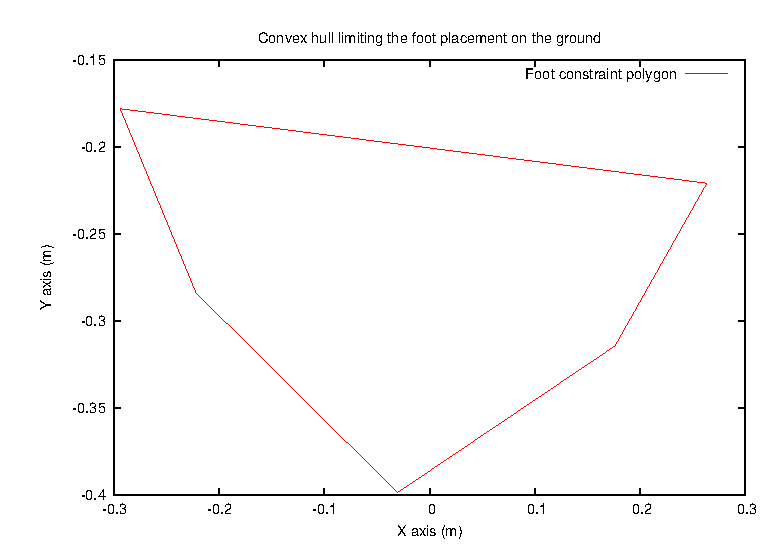
\includegraphics[width=15cm]{./figures/walking-without-thinking/ConvexHull}
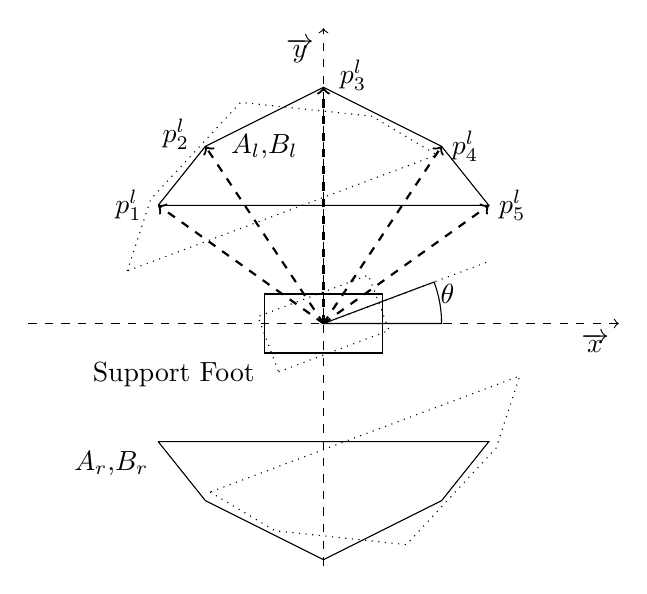
\begin{tikzpicture}[scale=0.075]
\draw [dashed][->](-50,0) -- (50,0) node [below left, black]{$\overrightarrow{x}$}; %x-axis
\draw [dashed][->](0,-41) -- (0,50) node [below left, black]{$\overrightarrow{y}$}; %y-axis
 %right support, left foot landing convexhull
\draw (-28,-20)--(-20,-30)--(0,-40)--(20,-30)--(28,-20)--(-28,-20) node [below left, black]{$A_r$,$B_r$} ;
 %left support, right foot landing convexhull
\draw (-28,20)--(-20,30)--(0,40)--(20,30)--(28,20)--(-28,20) node at (-10,30)[black]{$A_l$,$B_l$} ;
 %support foot
\draw (-10,-5)--(10,-5)--(10,5)--(-10,5)--(-10,-5) node [below left, black]{Support Foot} ;

% rotated support foot
\draw [dotted][cm={cos(\tetazero) ,sin(\tetazero) ,-sin(\tetazero) ,cos(\tetazero) ,(0.0 cm,0.0 cm)}]
(-10,-5)--(10,-5)--(10,5)--(-10,5)--(-10,-5) ;
% rotated axis
\draw [dotted][-][cm={cos(\tetazero) ,sin(\tetazero) ,-sin(\tetazero) ,cos(\tetazero) ,(0.0 cm,0.0 cm)}]
(0,0) -- (30,0) node [below left, black]{};
% angle
\draw (0,0) -- (18.727324381,7.02049297) arc (\tetazero:0:20) -- (0.0,0.0) node at (21,5) {$\theta$} ;
% rotated left support, right foot landing convexhull
\draw [dotted][-][cm={cos(\tetazero) ,sin(\tetazero) ,-sin(\tetazero) ,cos(\tetazero) ,(0.0 cm,0.0 cm)}]
(-28,20)--(-20,30)--(0,40)--(20,30)--(28,20)--(-28,20) ;
% rotated right support, left foot landing convexhull
\draw [dotted][-][cm={cos(\tetazero) ,sin(\tetazero) ,-sin(\tetazero) ,cos(\tetazero) ,(0.0 cm,0.0 cm)}]
(-28,-20)--(-20,-30)--(0,-40)--(20,-30)--(28,-20)--(-28,-20);

\draw [thick][dashed][->](0,0) -- (-28,20) node [black] at (-33.0,20.0){${p}_1^l$}; %y-axis
\draw [thick][dashed][->](0,0) -- (-20,30) node [black] at (-25.0,32.0){${p}_2^l$}; %y-axis
\draw [thick][dashed][->](0,0) -- (0.0,40) node [black] at (5.0,42.0){${p}_3^l$}; %y-axis
\draw [thick][dashed][->](0,0) -- (20,30) node [right, black]{${p}_4^l$}; %y-axis
\draw [thick][dashed][->](0,0) -- (28,20) node [right, black]{${p}_5^l$}; %y-axis

\end{tikzpicture}
